\documentclass[12pt]{article}
\usepackage{amsmath}
\usepackage{amssymb}
\usepackage{graphicx}
\usepackage{float}
\usepackage[margin=2cm]{geometry}
\usepackage[parfill]{parskip}
\usepackage{listings}
\usepackage{xcolor}
\usepackage{adjustbox}
\usepackage[style=numeric-comp,useprefix,hyperref,backend=bibtex]{biblatex}
\definecolor{dark-green}{RGB}{0,175,0}
\definecolor{dark-red}{RGB}{200,0,0}
\graphicspath{ {./pictures/} }
\addbibresource{report.bib}
\setcounter{tocdepth}{6}
\DeclareUnicodeCharacter{202F}{\,}
\begin{document}
	\title{NAML Project Report - Group 14\\\vspace{20pt}
		\Large{Music Genre Classification using}\\
		\large{k-Nearest Neighbours\\ Nearest Centroid\\ Multiclass SVM}\\
		\date{February 2022}
		\large{-\\}
		\large{by Silvia Marino (10688672) and Francesco Panebianco (10632465)\\}
		\small{prof. Edie Miglio e Francesco Regazzoni - Politecnico di Milano}
	}
	\maketitle
	\tableofcontents
	\newpage
	\section{Introduction}
	\paragraph{Scope}\mbox{}\\\newline
	The scope of this project is to create a music genre classifier using two machine learning methods: \textit{k-Nearest Neighbours} and \textit{Multiclass SVM}, which were assigned to our group. The project is part of the evaluation of the “Numerical Analysis for Machine Learning” course, taught in the first semester of the first year of Master’s Degree in Computer Science and Engineering at Politecnico di Milano. Given the similarities between \textit{k-Nearest Neighbours} and \textit{Nearest Centroid}, we chose to implement the latter as well, comparing its performance to the former, even though it is outside the specification of the project.\\ 
	
	\paragraph{The Dataset}\mbox{}\\\newline
	The dataset assigned to our project is the notorious \textit{GTZAN Genre Collection}\cite{marsyas}, which contains 100 different extracts from 10 different music genres. The dataset genres are: 
	
	\begin{itemize}
		\item Blues 
		\item Classical 
		\item Country 
		\item Disco 
		\item Hip Hop 	
		\item Jazz 
		\item Metal 
		\item Pop 
		\item Reggae 
		\item Rock 
	\end{itemize}

	As it can be seen, genres that share similarities are included in the dataset (e.g. Blues and Jazz), but also dramatically different types of music such as Rock and Classical, which we expect the algorithms to distinguish with higher precision.
	
	The dataset provides audio samples as \textit{.wav} files (\textit{Waveform Audio File Format}). WAV is the most common uncompressed audio file format in Microsoft Windows systems. It was developed by IBM and Microsoft, for storing an audio bitstream on PCs\cite{wave}.\\
	
	\begin{figure}[H]
		\hspace{100pt}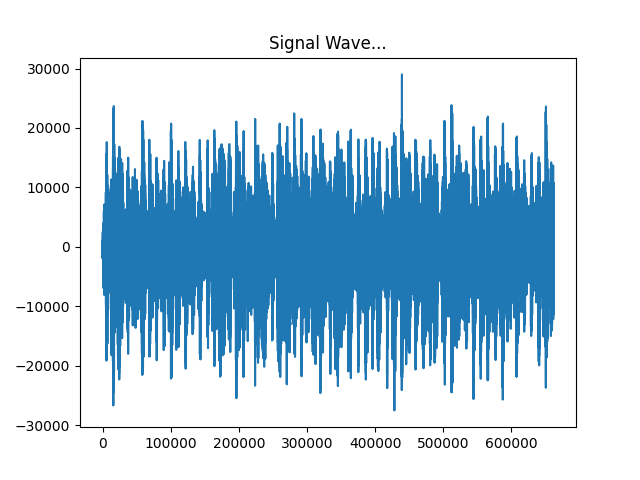
\includegraphics[scale=0.7]{waveform}
		\caption{Plotted waveform of blues.00000.wav}
	\end{figure}
	
	
	This file format can be imported in \textit{Python} by using the \textit{wave} module, which provides convenient functions to work with the WAV sound format. In our case, the audio samples are provided as 22050Hz Mono 16-bit 30 second tracks\cite{marsyas}, which are easily transformed into a numpy array of \textit{int16}.\\
	The picture above is the result of the following code:
	\begin{lstlisting}[language=Python]
		import wave
		import matplotlib.pyplot as plt
		import numpy as np
		
		test_file = wave.open('genres/blues/blues.00000.wav', 'rb')
		# Extract Raw Audio from Wav File
		signal = test_file.readframes(-1)
		signal = np.frombuffer(signal, dtype='int16')
		test_file.close()
		
		plt.figure(1)
		plt.title("Signal Wave...")
		plt.plot(signal)
		plt.show()
		
	\end{lstlisting}
	\newpage
	
	\paragraph{Feature Extraction}\mbox{}\\\newline
	For what concerns the features required to classify the genres, our first choice was the feature triplet of \textit{Zero Crossing Rate}, \textit{Average Energy} and \textit{Silent Ratio} as defined in one of the papers provided by the project specification \cite{comparison}. The extracted features were collected and exported in a csv file to avoid having to extract the feature multiple times, as the complete process took approximately 45 minutes on \textit{Google Colab}.\\
	
	\textbf{Zero Crossing Rate}\\
	It indicates the frequency of signal amplitude sign change, which is in some way related to the average signal frequency. In practice, it is a key feature to classify percussive sounds as it's often correlated with the beat. ZCR records how many waves have passed for a certain time, by averaging the sign changes in the signal amplitude. The implemented formula is as follows:
	
	\begin{equation}
		\text{ZCR}=\dfrac{\sum_{n=1}^{N-1}{\bigg|\text{sgn}\ x(n)-\text{sgn}\ x(n-1)\bigg|}}{2N}
	\end{equation}
	
	where sgn $x$ is the \textit{sign function}.\\
	
	\textbf{Average Energy}\\
	It indicates the loudness of the audio signal as a whole, being the average of the square amplitude of the audio signal.
	\begin{equation}
		\text{E}_\text{avg}=\dfrac{\sum_{n=0}^{N-1}{x(n)^2}}{N}
	\end{equation}
	In practice, it corresponds to the momentum or the force of the music within the time slice where it is measured. \\
	
	\textbf{Silent Ratio}\\
	It indicates the proportion of the sound piece that is considered to be \textit{silent}. Silence is defined as a period within which the absolute value of amplitude is below a certain threshold. If we indicate
	\begin{equation}
		SR = \dfrac{\sum_{x(n)<\text{thr}} 1}{N}
	\end{equation}
	In our implementation, silence threshold is derived from the average energy as follows...
	\begin{equation}
		\text{thr}=0.8\sqrt{E_\text{avg}}
	\end{equation}
	\newpage
	
	\paragraph{Dataset Visualization}\mbox{}\\\newline
	After exporting the feature dataset, we visualized it using built-in functions from \textit{pandas} and \textit{seaborn}. Full dataset visualization is available in a the Jupyter Notebook called\\ \textit{NAML\_Project\_Data\_Visualization.ipynb}.
	
	\begin{lstlisting}
    		       ZCR  AVERAGE_ENERGY  SILENT_RATIO
	count  1000.000000    1.000000e+03   1000.000000
	mean      0.103768    2.631159e+07      0.827613
	std       0.041886    2.396840e+07      0.024517
	min       0.021714    6.178678e+04      0.767521 
	25%       0.070328    9.781419e+06      0.810039
	50%       0.099618    1.834412e+07      0.824969
	75%       0.132136    3.768007e+07      0.842175
	max       0.275001    1.777716e+08      0.926341
	\end{lstlisting}
	
	\begin{figure}[H]
		\hspace{100pt}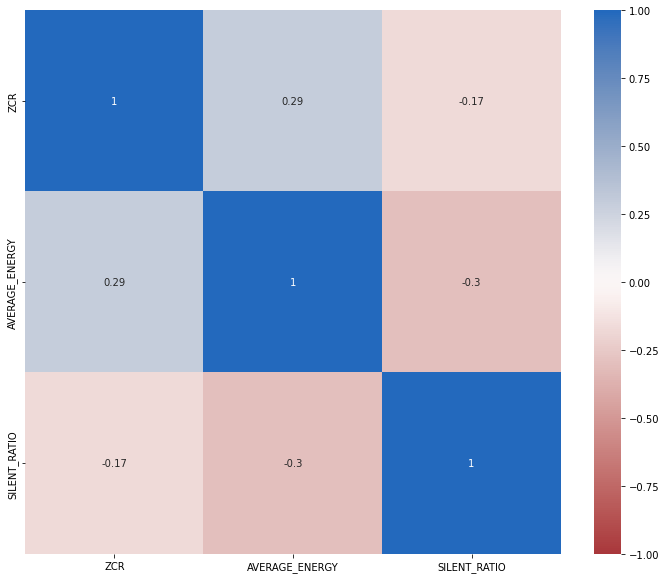
\includegraphics[scale=0.7]{visual_8_1}
		\caption{Annotated Heatmap of the correlation of extracted features}
	\end{figure}
	From this visualization, it is evident that the three features are independent enough to be non-redundant in the classification. 
	
	\begin{figure}[H]
		\hspace{40pt}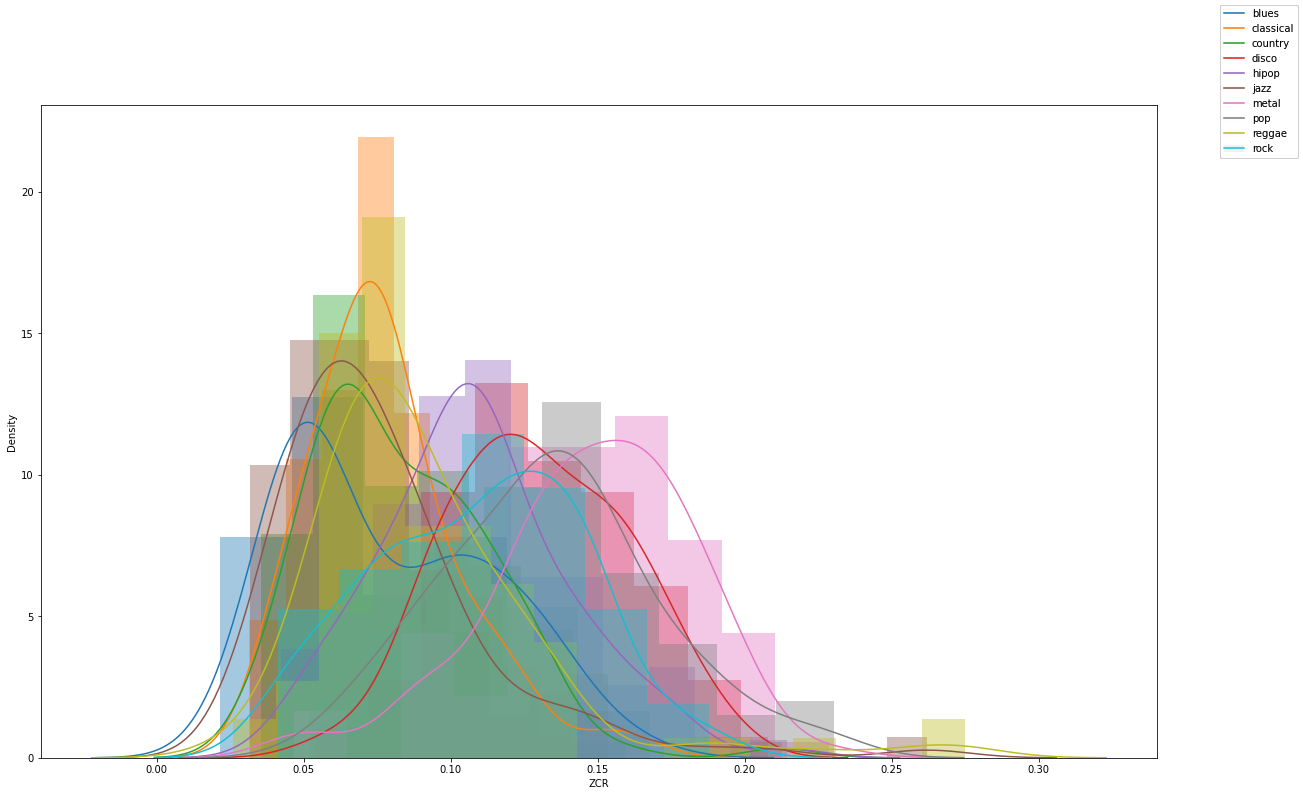
\includegraphics[scale=0.55]{visual_4_1}
		\caption{Distribution Plot of ZCR feature}
	\end{figure}
	
	\begin{figure}[H]
		\hspace{40pt}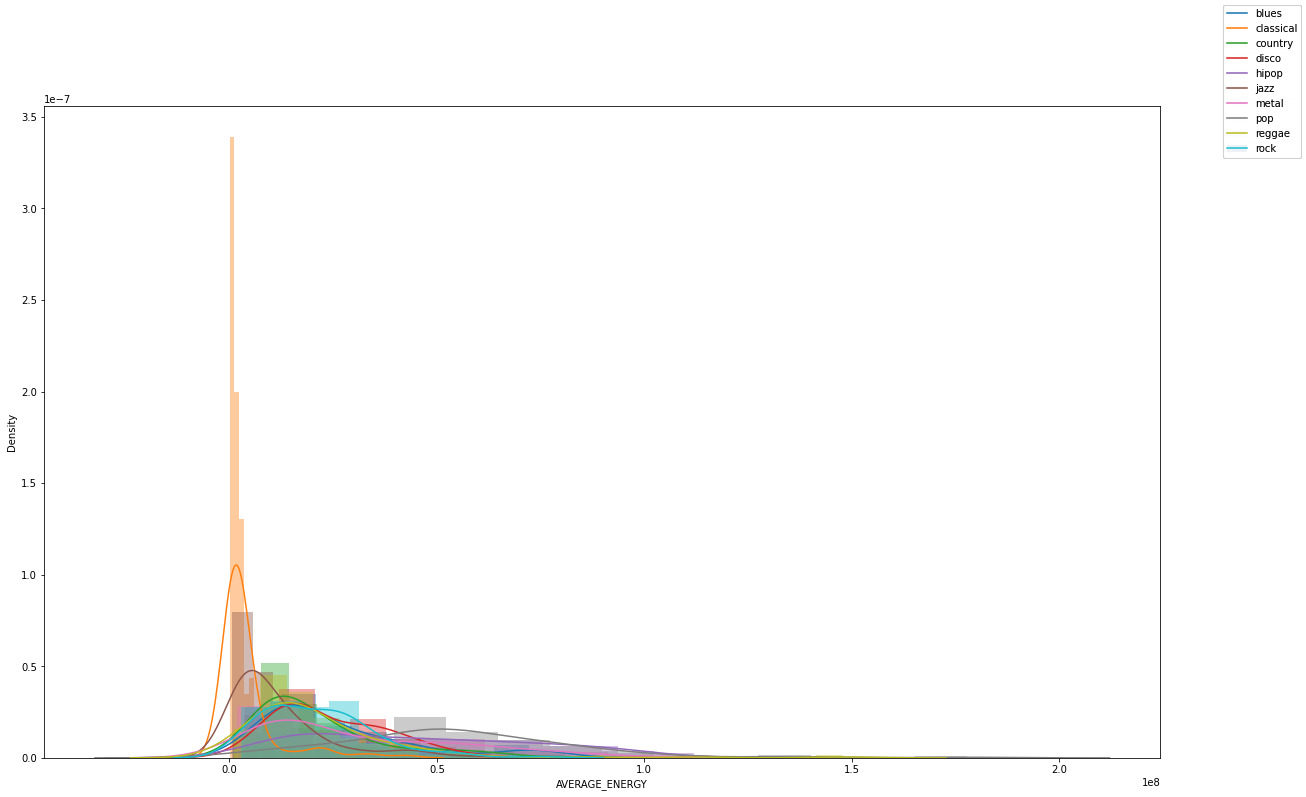
\includegraphics[scale=0.55]{visual_5_1}
		\caption{Distribution Plot of Average Energy feature}
	\end{figure}
	
	\begin{figure}[H]
		\hspace{40pt}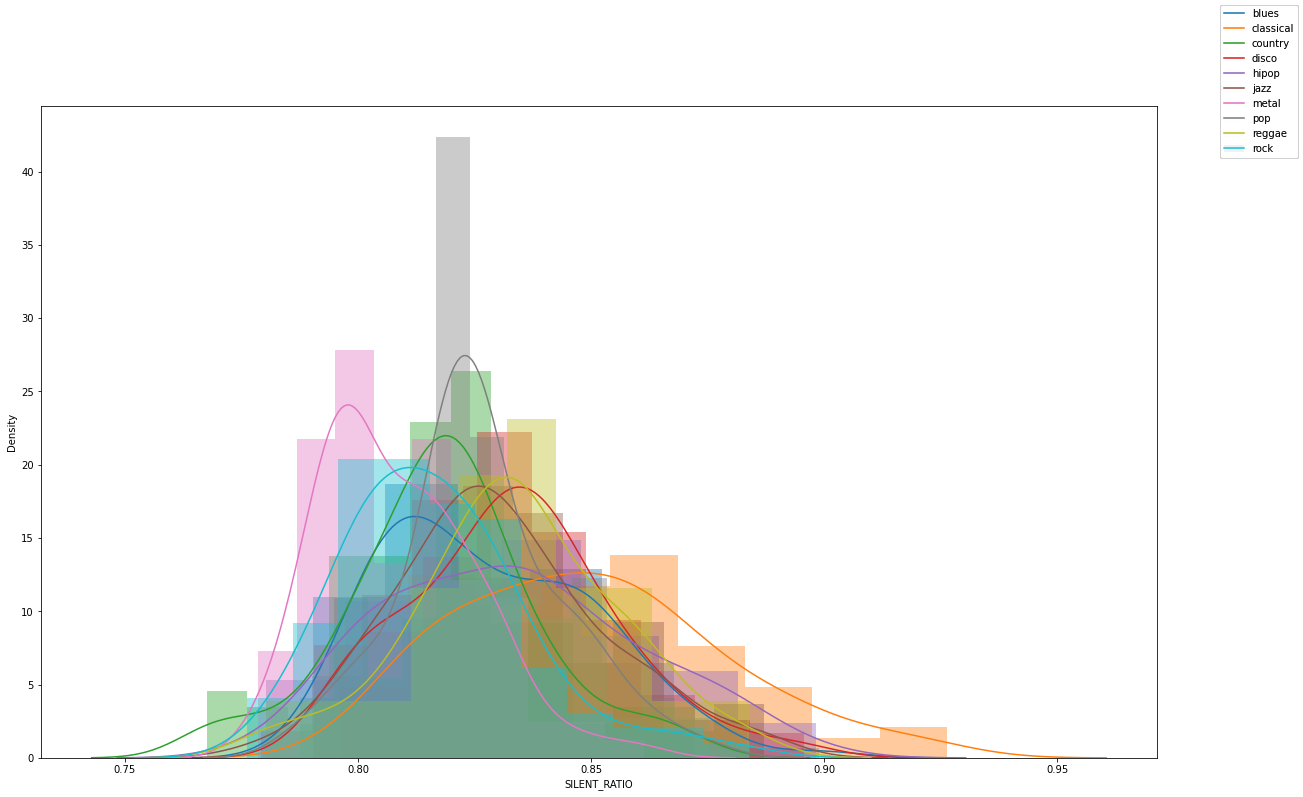
\includegraphics[scale=0.55]{visual_6_1}
		\caption{Distribution Plot of Silent Ratio feature}
	\end{figure}

	\paragraph{Alternative Feature Set: Mel-Frequency Cepstral Coefficients}\mbox{}\\\newline
	The second paper provided by the project specification \cite{classification} mentioned the possibility of using \textit{Mel-Frequency Cepstral Coefficients} as features for music genre classification.
	
	The \textbf{Mel-frequency Cepstrum} (MFC) is a representation of the short term power spectrum. The \textbf{Mel-frequency Cepstral Coefficients} (MFCCs) collectively make up an MFC. A Cepstrum is defined as a non-linear spectrum-of-a-spectrum.
	
	The peculiarity of an MFC with respect to a generic cepstrum is, as the name suggests, the usage of the \textit{Mel-frequency Scale}, which emulates the human hearing response more closely than the linearly spaced frequency bands used in the normal spectrum.
	
	MFCC extraction is a relatively standardized algorithm, so we've chosen a popular python library to aid us in the extraction: \textit{librosa}. As the library source code shows \cite{librosarepo}, the implemented extraction procedure is as follows:
	\begin{enumerate}
	\item Since a time series is provided, the spectrogram of the signal is computed.
	\item The spectrogram is mapped to the mel scale
	\item The $\mathbf{\log}$ of the result is taken (dB conversion)
	\item The \textit{Discrete Cosine Transform} is applied
	\end{enumerate}
	
	The Librosa implementation also supports a final processing step: Sinusoidal Liftering, which is reportedly considered beneficial to speech recognition applications. Since this is outside the scope of the classifier, no Liftering was applied.
	
	The input signal is automatically divided into a certain number of windows, each with their MFCCs, most applications can deal with the first 13 MFCCs, as they carry the most relevant information for the section of the spectrum that can be heard by the human ear.
	\begin{figure}[H]
		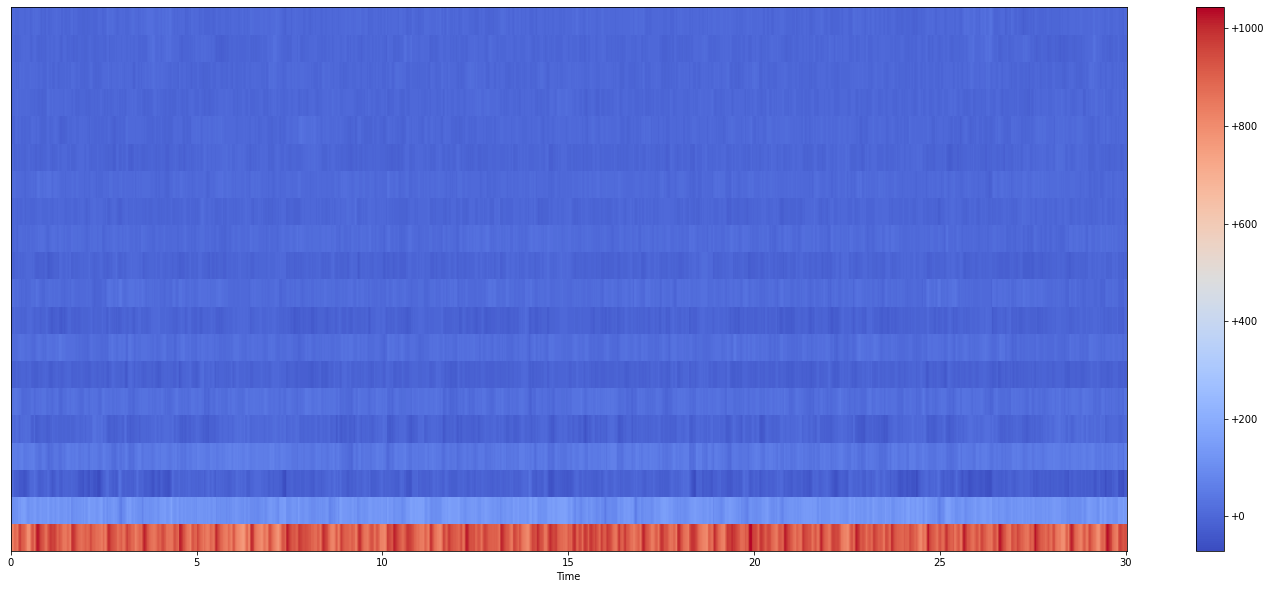
\includegraphics[scale=0.4]{mfcc_spectrogram}
		\caption{Mel-Frequency Cepstral Coefficents spectrogram of \textit{blues.00000.wav}}
	\end{figure}
	
	The resulting MFCCs of the signal are returned in a matrix with rows corresponding to the 13 coefficients and columns corresponding to all windows of the original signal. This is a dynamic representation of the signal, but we need to make a choice to extract static features for our classifier. We first tried averaging the coefficients across all windows, but their correlation was too high. In the end we noticed that picking coefficients from a random window of the song extract gave us a solid feature set with low enough correlation for the classifier to perform in a satisfactory manner.
	
	Librosa also allows for the computation of local estimates of n-order derivatives for MFCCs using the \textit{librosa.feature.delta} function. We also included these features (namely order 1 and 2 deltas) from the same random window as the coefficients. 
	
	A specific Jupyter Notebook named \textit{NAML Project Mel-frequency cepstrum.ipynb} handles the visualization and generation of the MFCC data for the dataset assigned to this project (the exported feature set is called \textit{mfcc\_dataset.csv}).
	
	\newpage
	
	\section{Classifiers}
	\paragraph{Distance Based Methods}\mbox{}\\
	In this paragraph we will explore the classifiers using the feature triplet (ZCR, Avg. Energy and Silent Ratio) using \textit{k-Nearest Neighbours} and \textit{Nearest Centroid}. The performance of both classifiers has been evaluated for different subsets of genres and using three different distance functions. Inspiration for the distance functions was taken from a recent computer science project work\cite{distances}. In the following formulas $\mathit{x}$ is the current sample, $\mathit{y}$ is the current centroid / training sample:
	\begin{itemize}
		\item \textbf{Euclidean Distance}:\\
		\begin{align}
			d(x,y)=\sqrt{\sum_{i=1}^n{(y_i-x_i)^2}}
			\begin{gathered}
				\hspace{50 pt}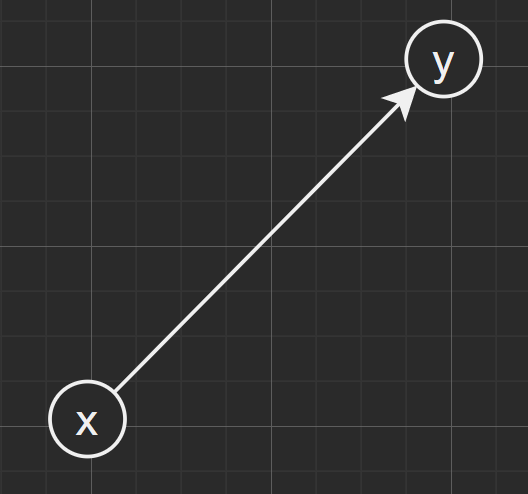
\includegraphics[width=0.2\linewidth]{dist_euclidean}
			\end{gathered}
		\end{align}

		\item \textbf{Manhattan Distance}:\\
		\begin{align}
			d(x,y)=\sum_{i=1}^n{\big|y_i-x_i\big|}
			\begin{gathered}
				\hspace{67 pt}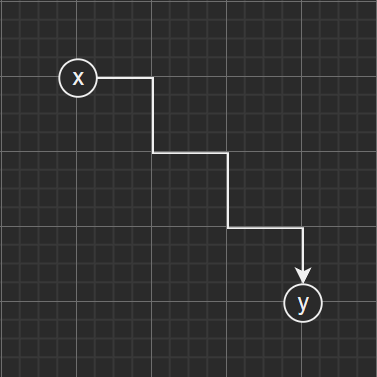
\includegraphics[width=0.2\linewidth]{dist_manhattan}
			\end{gathered}
		\end{align}
		\item \textbf{Chebyshev Distance}:\\
		\begin{align}
			d(x,y)=\max_i{\big|y_i-x_i\big|}
			\begin{gathered}
				\hspace{67 pt}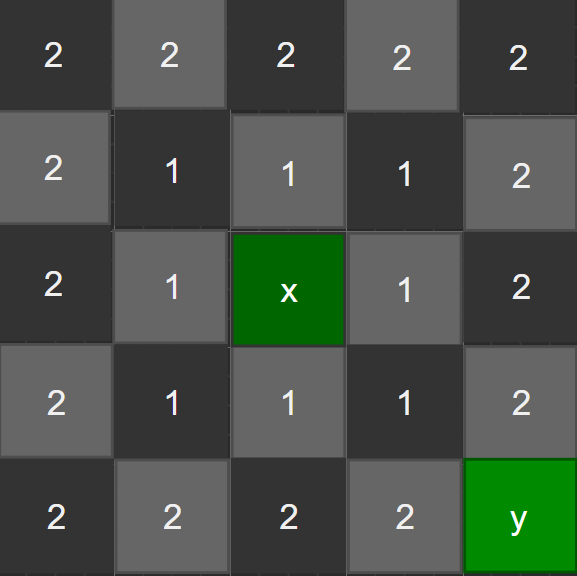
\includegraphics[width=0.2\linewidth]{dist_cheb}
			\end{gathered}
		\end{align}
	\end{itemize}
	\mbox{}\newpage
	\subparagraph{k-Nearest Neighbours Classifier}\mbox{}\\\newline
	The implementation of the \textit{k-Nearest Neighbours Classifier} was developed and tested in the jupyter notebook \textit{NAML\_Project\_k\_Nearest\_Neighbours.ipynb} and was later ported to a standalone python script to be callable as a module (/knn/k\_nearest\_neighbours\_classifier.py).\\
	We calculate the distances between the input and all the data of the genres previously selected, we then store in an array the k minimum distances and the classes to which they belong. If k is greater than one, we count the occurrences of each class present in the k nearest points. In case of a tie, we return the class with the smallest distance.
	\begin{figure}[H]
		\hspace{70pt}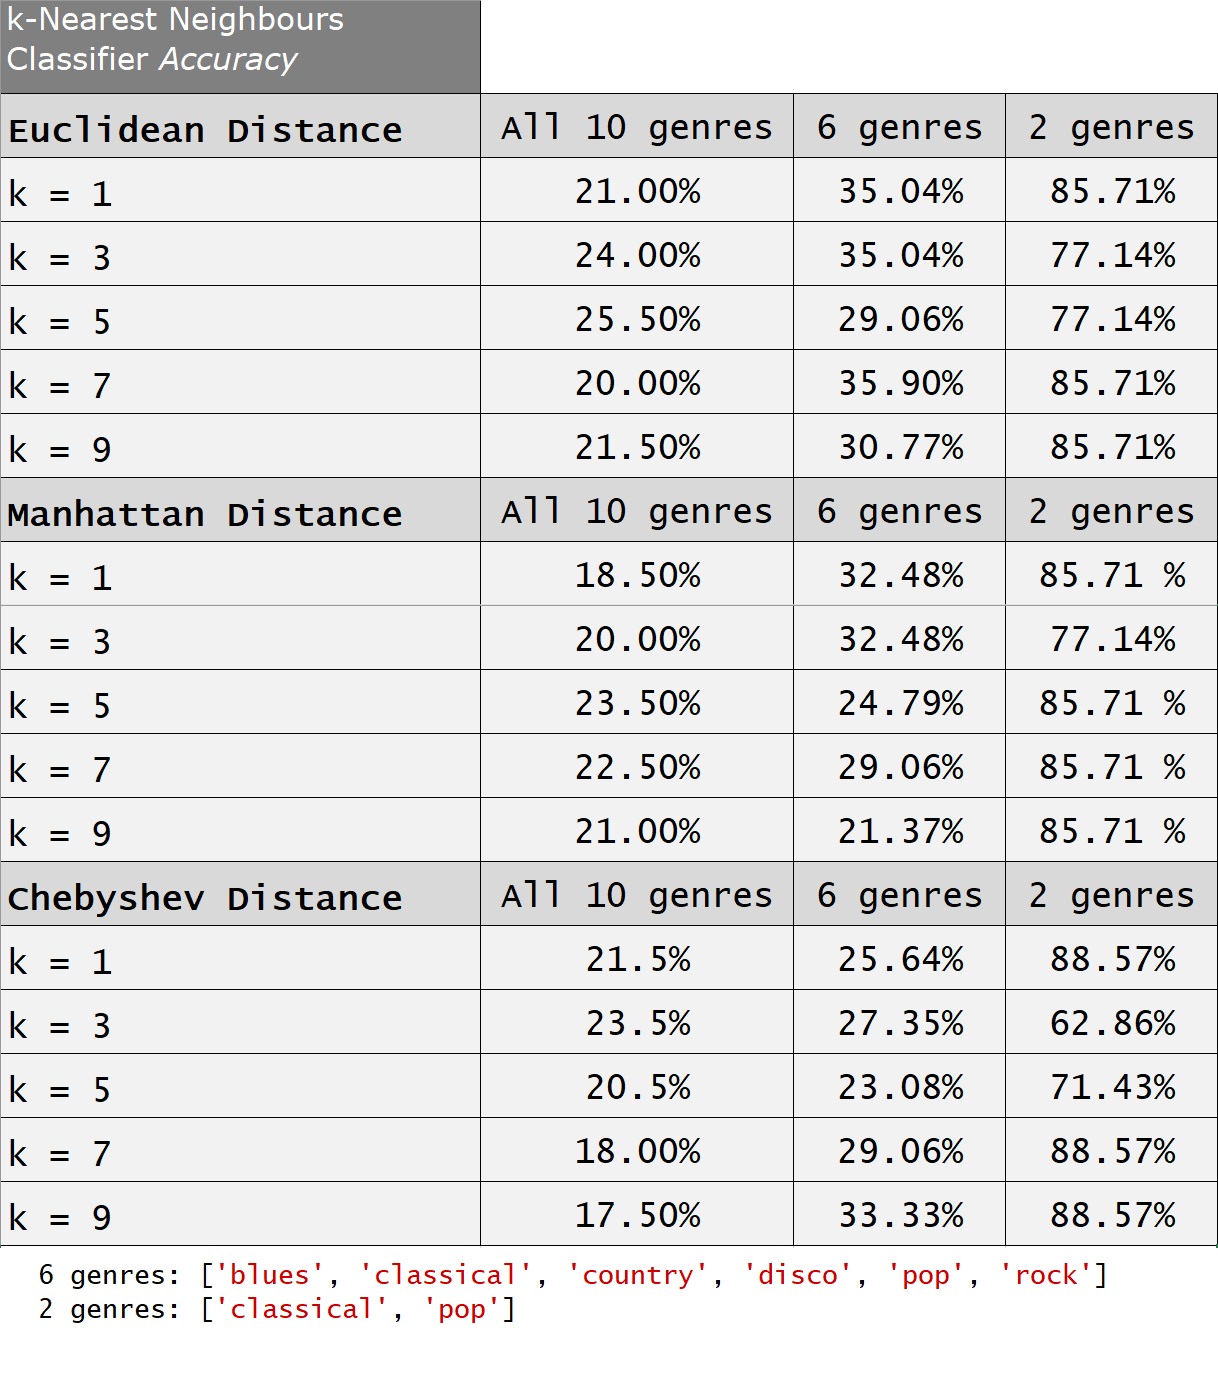
\includegraphics[scale=0.5]{knn_acc}
		\caption{Accuracy table for k-Nearest Neighbours}
	\end{figure}
	\newpage
	\subparagraph{Nearest Centroid Classifier}\mbox{}\\\newline
	The implementation of the \textit{Nearest Centroid Classifier} is straightforward enough. It was developed and tested in the jupyter notebook \textit{NAML\_Project\_Nearest\_Centroid.ipynb} and was later ported to a standalone python script to be callable as a module (/nearest\_centroid/nearest\_centroid\_classifier.py). 
	To determine the centroid for each class, the training set is filtered and the mean of each feature is computed. A list called \textit{centroids} collects the centroid vectors after their computation.
	
	\begin{figure}[H]
		\hspace{50pt}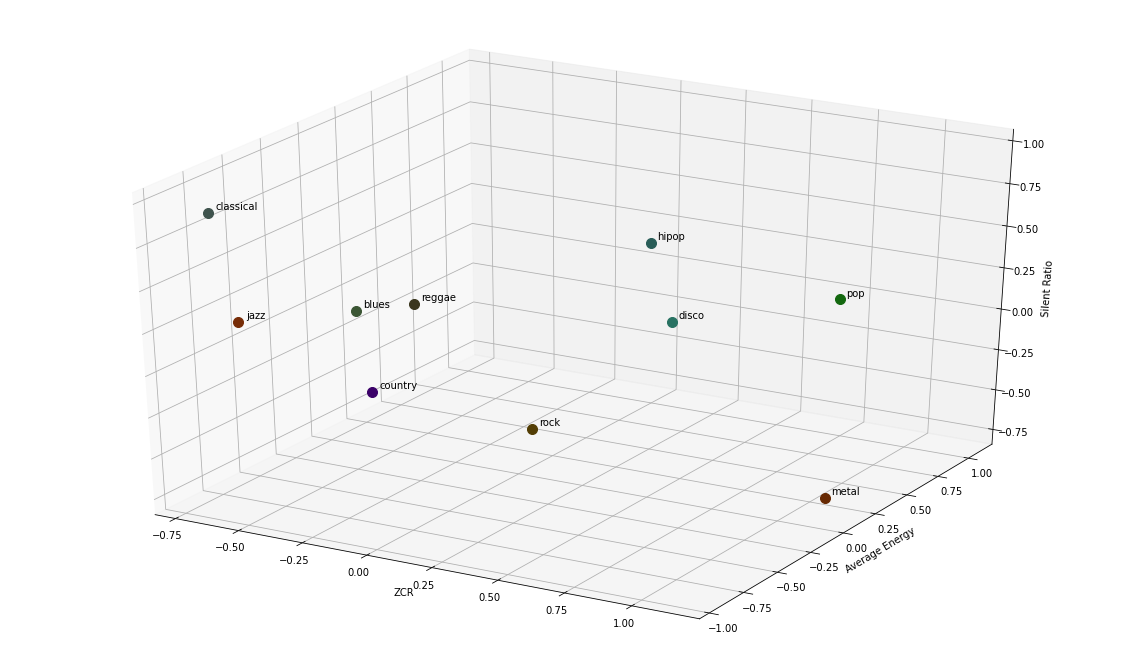
\includegraphics[scale=0.4]{centroids_plot}
		\caption{3d scatterplot of class centroids}
	\end{figure}

	To classify the genre given the input and the possible genres to classify to, the algorithm determines the closest centroid among the available ones using the distance function passed as a parameter in the \textit{classify} function. Here are the resulting classification accuracies:
	\begin{figure}[H]
		\hspace{70pt}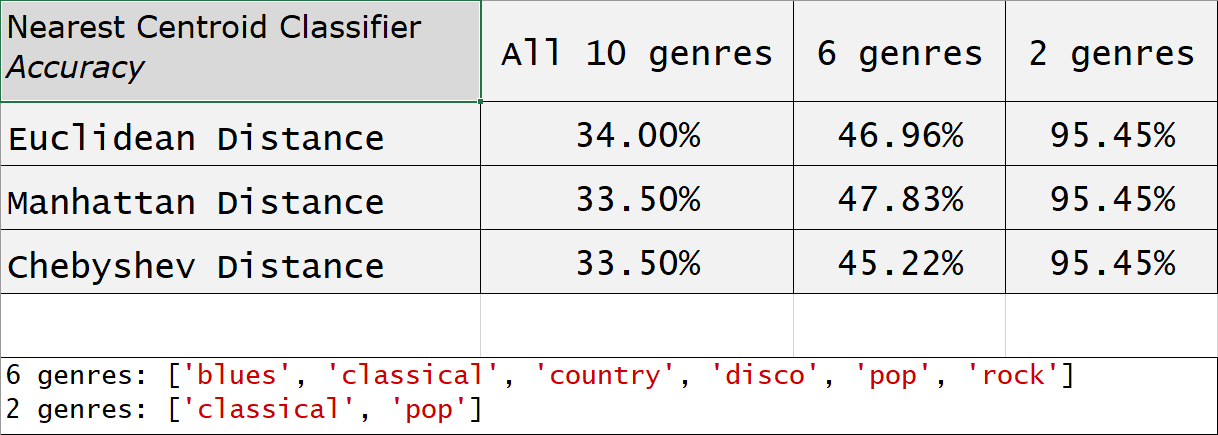
\includegraphics[scale=0.5]{nc_acc}
		\caption{Classification accuracy for each distance/genre set}
	\end{figure}
	
	\paragraph{Multiclass SVM Classifiers}\mbox{}\\\newline
	The implementation of a \textit{Support Vector Machine} classifier can be accomplished in a variety of different ways. To explore them before moving to the full Multiclass application, we created a Jupyter Notebook called \textit{NAML\_Project\_Experiments.ipynb}. After testing the binary classification performance, we adapted the code for the multi-class case, exploring both the \textit{One-To-Rest} strategy and the \textit{One-To-One} strategy.
	\subparagraph{Building Blocks}\mbox{}\\\newline
	The implementation of a Support Vector Machine problem can be either derived from the primal or the dual formulation.
	
	\textbf{Primal Formulation - Hard Margin}\\
	The problem of computing the \textit{maximum-margin hyperplane} exploiting \textit{support vectors} (samples from either class lying on the "gutter" that separates the two classes) can be formulated as follows:\\
	\begin{align}
		\min_{w,b} \Vert w \Vert &&
		\text{s.t.}\ \ y_i(w^Tx-b)\ge 1
	\end{align} 
	Where $\mathbf{y_i =\pm 1}$ is the label of the class corresponding to sample $\mathbf{x}$.\\
	
	\begin{figure}[H]
		\hspace{120pt}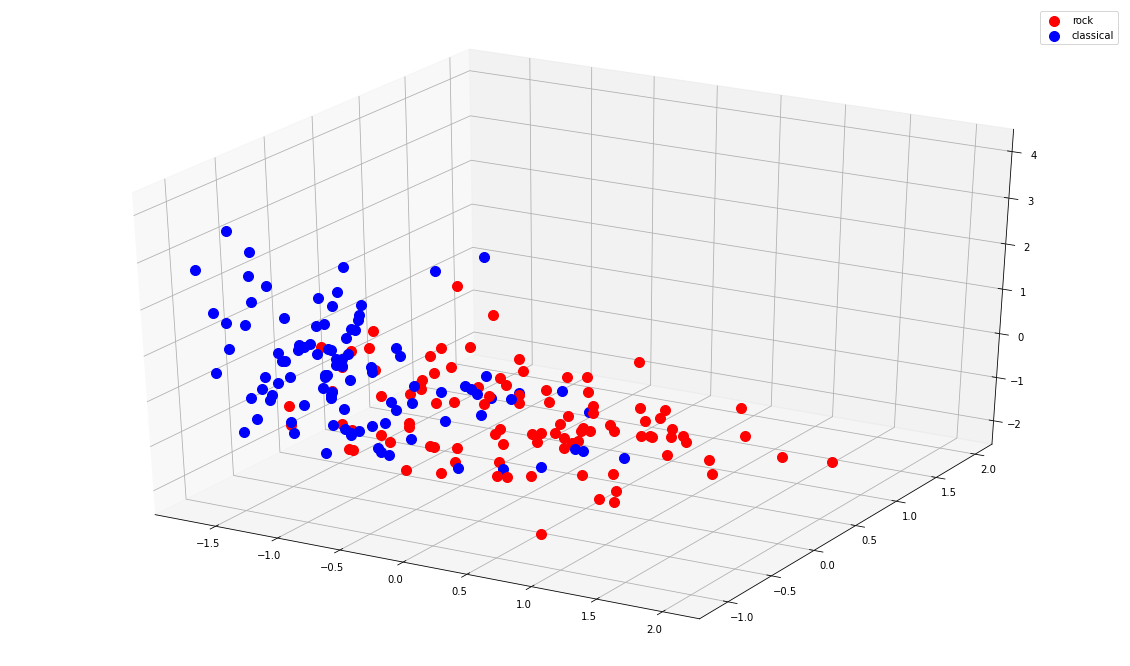
\includegraphics[scale=0.2]{exp1_legend}
		\caption{3d scatterplot of rock and blues samples}
	\end{figure}
	
	Unfortunately, our samples are not linearly separable using a hard-margin, so this basic form of classification was not chosen.\newpage
	
	\textbf{Primal Formulation - Soft Margin}\\
	The soft-margin formulation involves the usage of the \textbf{hingeloss} function, which makes the optimization problem become
	
	\begin{align}
		\min_{w,b}\ \ \ \dfrac {1}{n} \sum_{i=1}^n{\max{\Big(0,1-y_i(w^Tx-b)\Big)}}
	\end{align}

	The optimization problem is unconstrained, which enables us to apply the \textit{Gradient Descent} method, particularly appropriate considering the convexity of the function. Most soft-margin implementations also feature a \textit{penalization} term, but in our implementation such parameter ended up decreasing the accuracy. Hence, we decided to remove it.
	
	\begin{figure}[H]
		\hspace{25pt}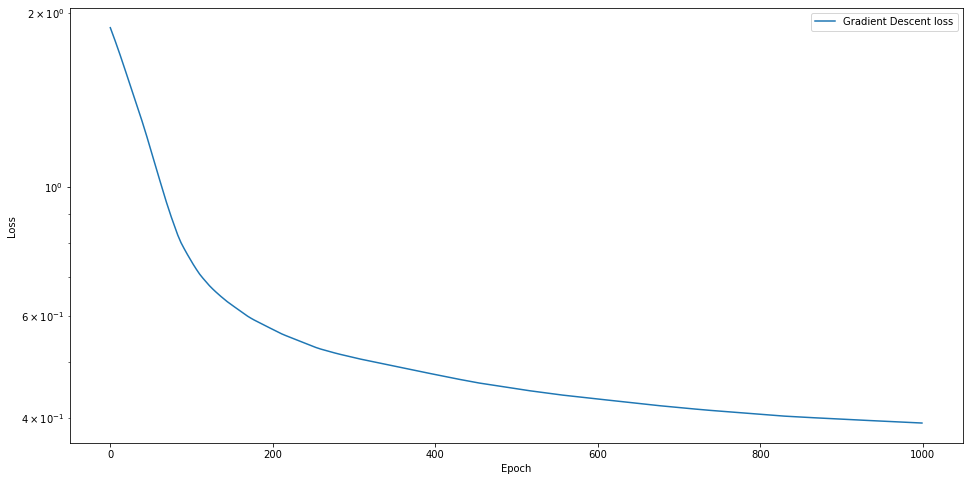
\includegraphics[scale=0.44]{gd1}
		\caption{Gradient Descent hingeloss history on rock/classical margin}
	\end{figure}
	\begin{figure}[H]
		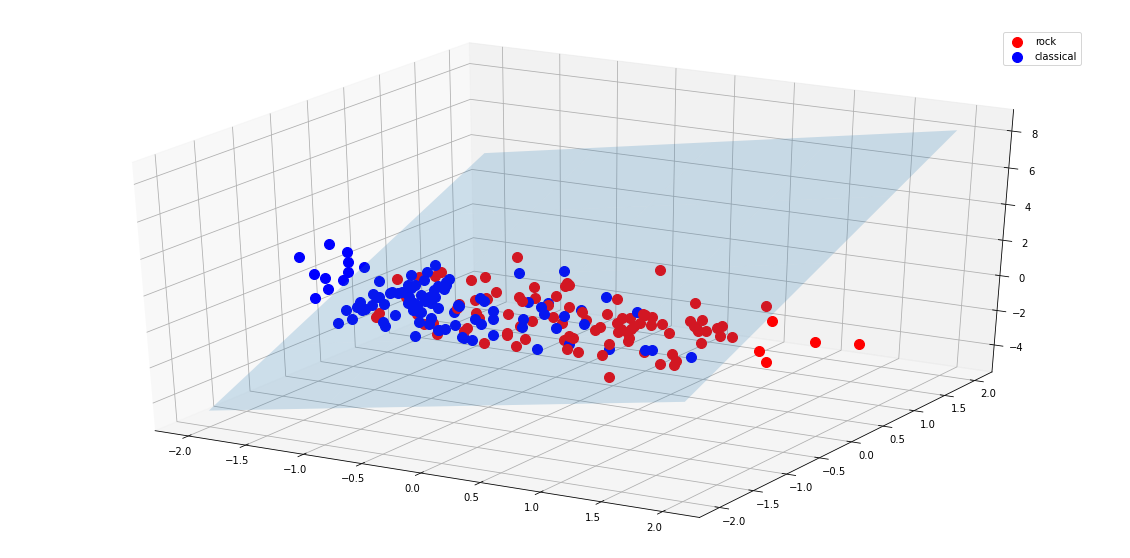
\includegraphics[scale=0.4]{plane1}
		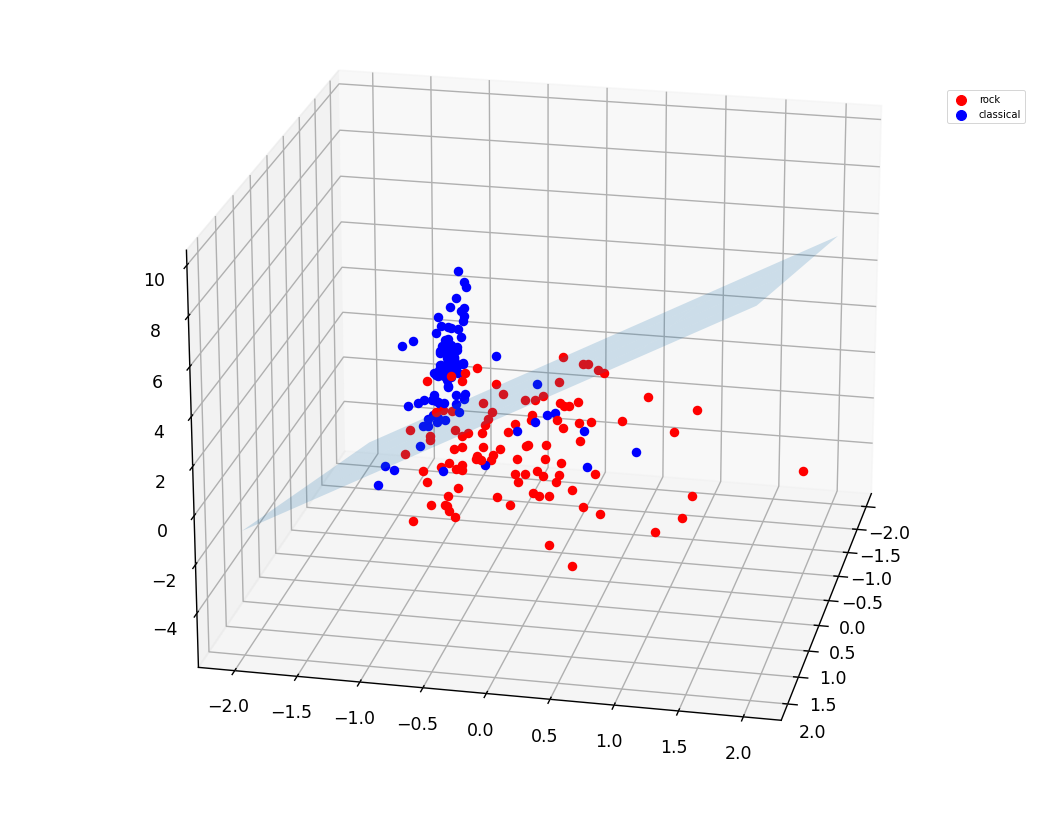
\includegraphics[scale=0.4]{plane1_side}
		\caption{Plots of the hyperplane corresponding to the optimal parameters (two different rotations of the point of view)}
	\end{figure}

	\textbf{Primal Formulation - Soft Margin with Feature Map}\\
	Before trying the dual formulation, which allows the usage of the Kernel Trick for non-linear classification margins, we tried a simple quadratic \textit{feature map} to be applied to the primal formulation. This way, the three samples (ZCR, average energy and silent ratio) are mapped to a higher dimensional feature space.
	\begin{align}
		\phi(x_1, x_2, x_3) &= \begin{bmatrix}
			x_1 \ \ \
			x_2 \ \ \
			x_3 \ \ \
			x_1^2 \ \ \
			x_2^2 \ \ \
			x_3^2 \ \ \
			x_1x_2 \ \ \
			x_2x_3 \ \ \
			x_1x_3
		\end{bmatrix} ^T
	\end{align}

	\begin{figure}[H]
		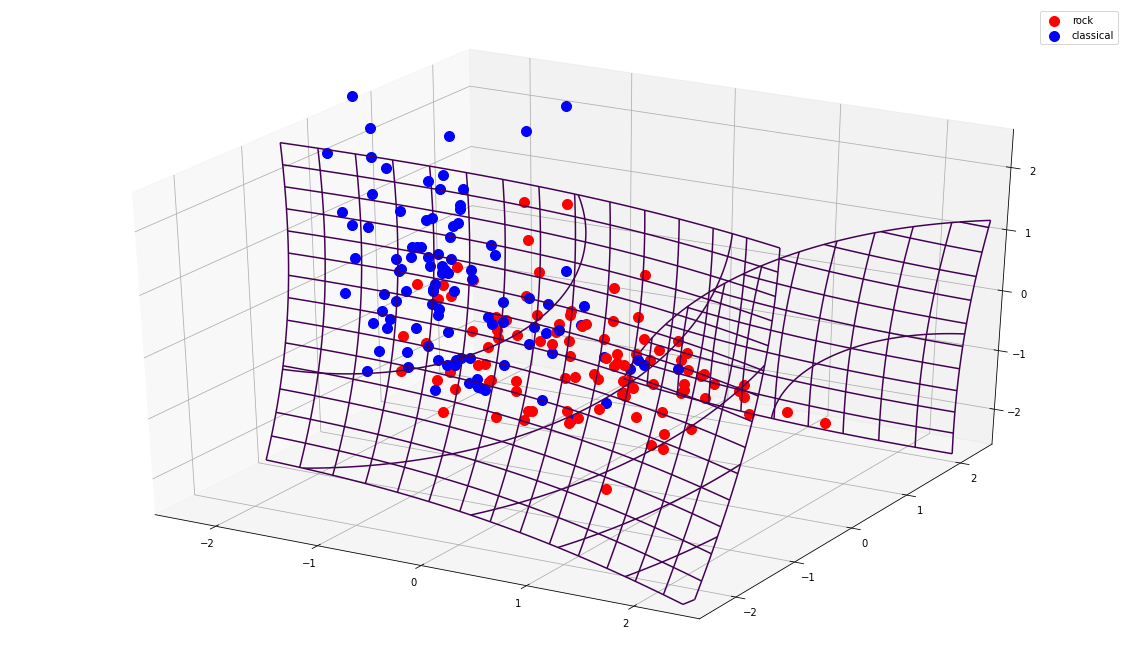
\includegraphics[scale=0.4]{quad_feat}
		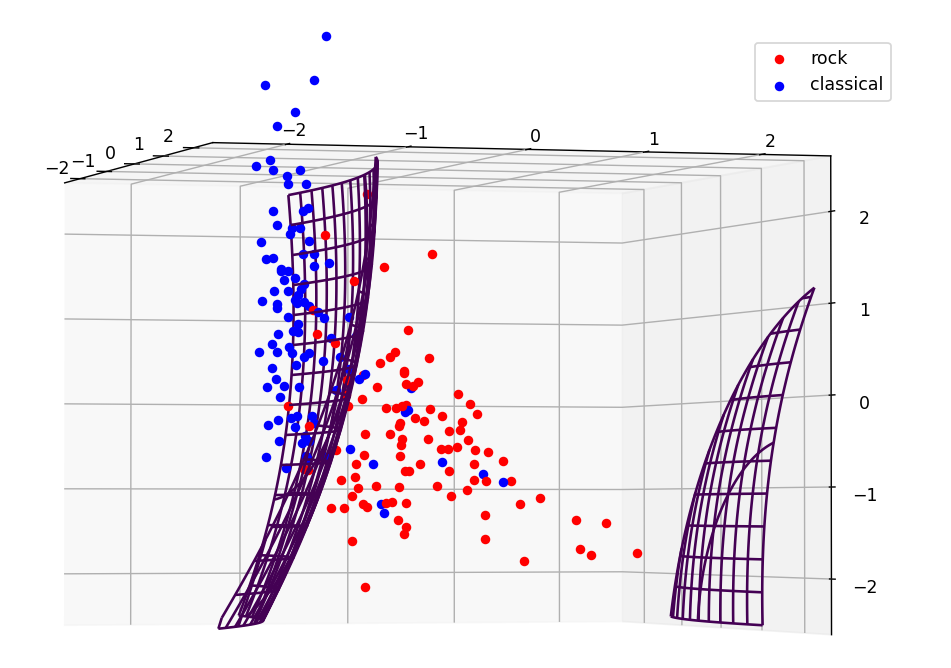
\includegraphics[scale=0.4]{quad_feat_side}
		\caption{Plots of the non-linear margin corresponding to the optimal parameters (two different rotations of the point of view)}
	\end{figure}
	
	\textbf{Dual Formulation - Linear Margin}\\
	The dual formulation of the SVM is easily obtained from the soft-margin primal formulation by using \textit{Lagrangian Multipliers...}
	\begin{align}
		\max_{c1,\dots, c_n}\ \ \ \sum_{i=1}^n{c_i} - \dfrac 1 2 \sum_{i=1}^n{\sum_{j=1}^n{c_i c_j y_i y_j x_i^Tx_j}} &&
		\nonumber \text{s.t.} \ \ \sum_{i=1}^n{c_iy_i} = 0\ \ \ \land \ \ c_i \ge 0
	\end{align}
	This time the optimization problem is constrained, so we had to use a \textit{Quadratic Programming} library available for python. We ended up using \textit{scipy.optimize}. Since the only constraint on the decision variable is linear, the computation of an iteration did not require the hessian, which was hardcoded to zero. The parameters of the optimization were method='trust-constr' (constrained minimization of scalar function) and jac='2-point' which enables the calculation of the jacobian of the constraint using finite differences \cite{docscipyopt}. Of course, since the dual formulation is a maximization problem, the objective function has to be multiplied by $\mathbf{-1}$ before being fed to the \textit{scipy.optimize.minimize} method.\\
	
	After running the computation, weights and bias can be derived from the following expressions
	
	\begin{align}
		w = \sum_{i=1}^n{c_iy_ix_i}&&
		b = w^Tx_i-y_i \ \ \text{for any } i\ \text{such that}\ x_i\ \ \text{lies on the margin}\  (c_i>0)
	\end{align}
	
	\textbf{Dual Formulation - Kernel Trick}\\
	The kernel trick can intuitively be applied to the objective function by replacing the dot product of two samples $\mathbf{x_i^Tx_j}$ with the kernel function $\mathbf{K(x_i,x_j)}$. The choice of the kernel function itself, unfortunately, was constrained by the performance of its computation. While a polynomial kernel was fast due to the matrix optimizations of \textit{numpy}, a gaussian kernel was found expensive. The following kernel had the best results in terms of classification accuracy:
	\begin{align}
		K(x_i,x_j)=(x_i^Tx_j+1)^3
	\end{align}
	The computation of the weights (multiplied by the kernel) and the bias is as follows:
	\begin{align}
		w_j^\phi = \sum_{i=1}^n{c_iy_iK(x_j,x_i)}&&
		b = w^\phi_i-y_i \ \ \text{for any } i\ \text{such that}\ x_i\ \ \text{lies on the margin}\  (c_i>0)
	\end{align}
	\textbf{From binary to multiclass}\\
	After testing all previously presented methods we noticed that the best results were provided by the
	classifiers that used \textit{Kernel Trick with Dual Formulation} and \textit{Feature Map with Primal Formulation}, so the first was chosen for the One-To-Rest classifier while the second was implemented in the One-To-One model.
	\subparagraph{One-To-Rest Classifier}\mbox{}\\\newline
	The implementation and testing of this  classifier was done in \textit{Google Colab} on the\\ \textit{NAML\_Project\_Multiclass\_OneToRest.ipynb} and was later ported to a python module for further usage.
	Even in this case, due to long execution
	time on \textit{Google Colab} (around 15 minutes), the usage of the standalone python module is discouraged, as it takes way more than 15 minutes to train the model on personal devices:
	\begin{figure}[H]
		\hspace{75pt}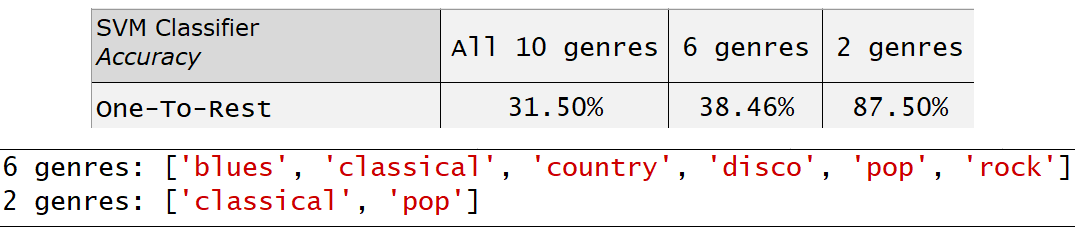
\includegraphics[scale=0.45]{svm_otr_acc}
		\caption{Classification accuracy for each genre set}
	\end{figure}
	Each binary classifier checks if the input passed belongs to a specific genre or not. Specifically, it calculates a “score” that is positive if the input is classified to belong to the considered genre, and negative otherwise.
	
	To decide which class to return, the one-to-rest classifier retrieves the highest score  among the genres considered during initialization.
	\newpage
	\subparagraph{One-To-One Classifier}\mbox{}\\\newline
	The implementation of the One-To-One classifier was done directly in \textit{PyCharm} to better exploit debugging tools in the implementation of the object oriented architecture of the module.
	
	Since the One-To-One classifier compares one genre to another, we decided to choose the actual predicted class using a \textbf{Binary Decision Tree}, which was implemented in a separate class using recursive algorithms. The amount of binary classifiers required for the multiclass problem of a given subset of $\mathit{n}$ genres is
	\begin{align}
		\text{\# classifiers} = \binom{n}{2} = \frac{n!}{2!(n-2)!}
	\end{align}

	Since the maximum number of genres to classify is 10, the maximum number of binary classifiers to be instantiated is 45.
	
	Once the class \textit{MulticlassSVM\_OTO} is instantiated, the \_\_init\_\_() method creates all combinations of classifiers and then recursively generates a binary decision tree, assigning a binary classifier to each node.
	\begin{figure}[H]
		\hspace{70pt}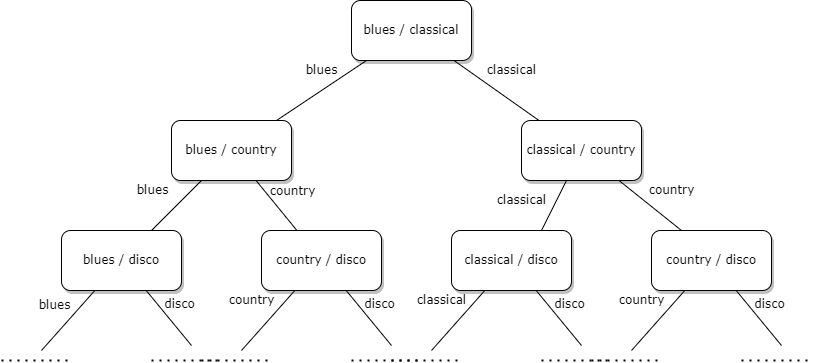
\includegraphics[scale=0.44]{decision_tree}
		\caption{Truncated example of decision tree as generated upon instantiation of DecisionBinaryTree}
	\end{figure}
	\begin{figure}[H]
		\hspace{80pt}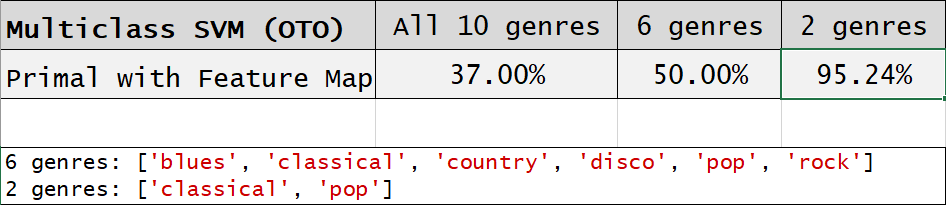
\includegraphics[scale=0.6]{svm_oto_acc}
		\caption{Classification accuracy for each genre set}
	\end{figure}
	\newpage
	
	\paragraph{Classification with MFCCs}\mbox{}\\
	Once the implementation of the classifiers with the feature triplet was completed, we started working with the same classifiers changing the feature set to the extracted MFCCs. All MFCC classifiers were implemented and tested on \textit{Google Colab} as jupyter notebook \textit{MFCC\_PCA.ipynb}. As the name of the notebook suggests, we were sure the usage of all 39 features without processing would have been redundant, so we started with a \textit{Principal Component Analysis} on the data.
	
	\begin{figure}[H]
		\hspace{70pt}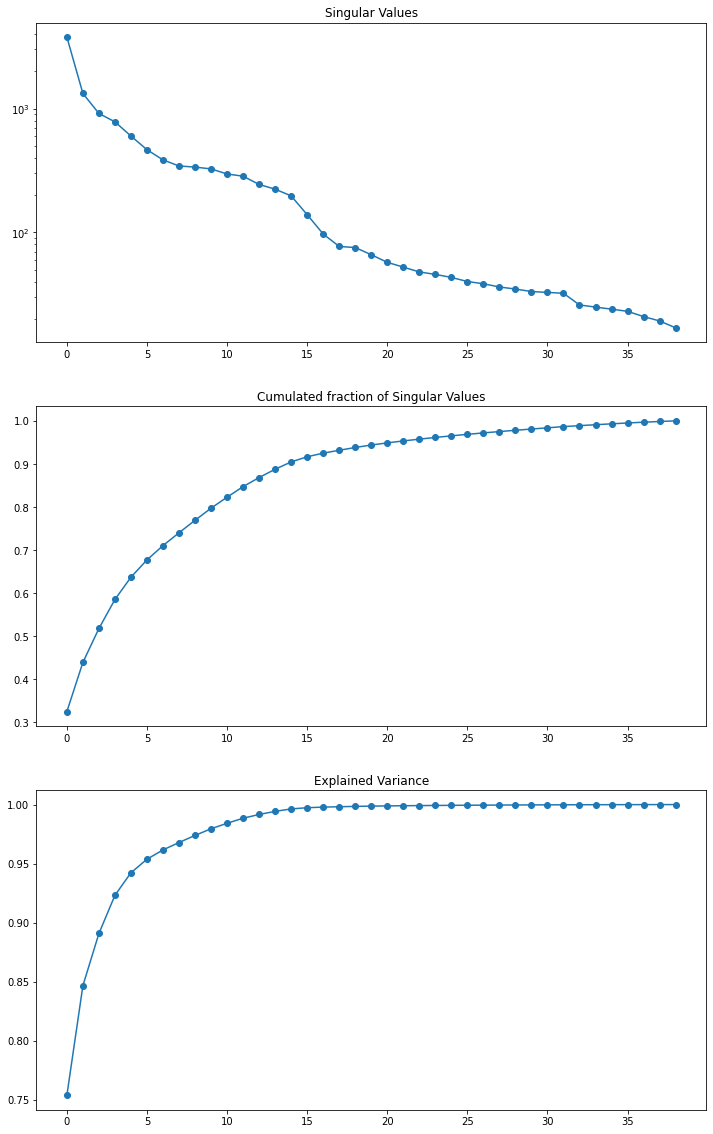
\includegraphics[scale=0.44]{mfcc_pca}
		\caption{Results of the Principal Component Analysis performed on the MFCC dataset}
	\end{figure}

	From the plots, it is evident that around 10 principal components provide more than enough of the variance of the original data to be used for classification.
	
	The accuracies for each technique are as follow:
	\begin{figure}[H]
		\hspace{120pt}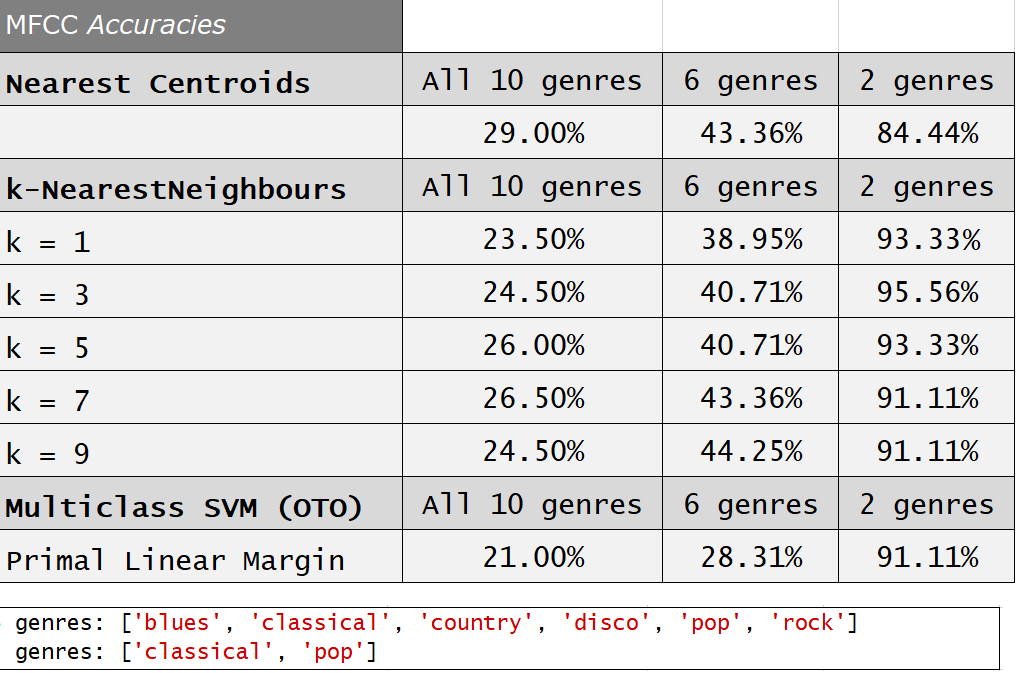
\includegraphics[scale=0.44]{mfcc_acc}
		\caption{Accuracies of classification with MFCC principal components}
	\end{figure}
	Considering the training time for the One-To-Rest classifier is way too long and the classification performance is poor, we did not include it in the MFCC classifiers notebook.
	Also, given that this alternative feature set does not improve accuracy compared to the feature triplet described before, we decided not to port the classification code to standalone python classes.
	\newpage
	
	\paragraph{Modules User Guide}\mbox{}\\
	In this paragraph we will explain how to use the standalone python modules we developed. Some examples of the usage of the following classes and functions are available in the \textit{tests} folder.
	
	\textbf{Feature Extraction Modules}\mbox{}\\
	- ./feat\_ext/sample\_processing.py
	
	\begin{lstlisting}[language=Python]
	# Used to load a wav audio signal located in path and of
	# type dtype (e.g. int16, int32, ...)
	load_audio_signal(path, dtype)
	
	# Takes a audio signal and a sample rate returns a 30 sec extract
	# taken from the center of the signal
	select_30sec_extract(signal, sampling_rate)
		
	# Takes a audio signal and returns the feature triplet
	# ZCR, avg_energy, silent_ratio as SEPARATE variables
	get_feature_triplet(signal)
	
	
	# Given a pandas dataframe of the extracted feature sets, returns
	# dataset_train, labels_train, dataset_valid, labels_valid
	# (in this exact order)
	get_normalized_train_valid_sets(data:pd.DataFrame, feature_count=3)
	\end{lstlisting}

	- ./feat\_ext/full\_feature\_extraction.py
	
	\begin{lstlisting}[language=Python]
	# Given an audio signal, returns its Zero Crossing Rate value
	zero_crossing_rate(signal)
		
	# Given an audio signal, returns its Average Energy value
	average_energy(signal)
		
	# Given an audio signal, returns its Silent Ratio value
	silent_ratio(signal)
		
	# Creates the full feature triplet set for the GTZAN dataset
	# given the path to the genres folder and saves it in a file
	# called 'new_dataset.csv' in the same folder as the module
	create_dataset(path_to_genres_folder)
	\end{lstlisting}
	\newpage
	\textbf{Utils for the distance based classifiers}\mbox{}\\
	- ./utils/distances.py
	\begin{lstlisting}[language=Python]
	# Returns the Manhattan Distance given x
	# Assumption (x already contains the difference between the
	# label and the prediction)
	manhattan(x)
	
	# Returns the Chebyshev Distance given x
	# Assumption (x already contains the difference between the
	# label and the prediction)
	chebyshev(x)
	\end{lstlisting}
	
	\textbf{k-Nearest Neighbours Classifier Module}\mbox{}\\
	- ./knn/k\_nearest\_neighbours\_classifier.py
	\begin{lstlisting}[language=Python]
class kNearestNeighboursClassifier:
	__init__() takes no parameters
	
	# Trains the k-Nearest Neighbours Classifier given
	# the training_set and the training_labels
	'''
	WARNING: dataset and labels are the COMPLETE dataset, even if you
	want to classify less than 10 genres
	'''
	self.train(training_set, training_labels)
	
	# Returns the name of the predicted genre given the
	# input sample, the list of possible genres,
	# the distance function and the number of
	# samples to check the distance from
	self.classify(input, genres_to_classify=genre_names, 
		distance=np.linalg.norm, k=1)
	
	# Returns the confusion matrix (always 10x10)
	# of the validation set and validation_labels
	# given the list of possible genres, the distance function
	# and the number of samples to check the distance from
	self.confusion_matrix(validation_set, validation_labels,
		genres_to_classify=genre_names, distance=np.linalg.norm,k=1)
	
	# Returns the accuracy of the classifier given a confusion matrix
	@staticmethod
	compute_accuracy_from_matrix(c_mat)
	
	# Returns the accuracy of the classifier given
	# the validation set and the validation labels
	self.compute_accuracy(dataset_validation, labels_validation)
	\end{lstlisting}
	\newpage
	\textbf{Nearest Centroid Classifier Module}\mbox{}\\
	- ./nearest\_centroid/nearest\_centroid\_classifier.py
	\begin{lstlisting}[language=Python]
class NearestCentroidClassifier:
	__init__() takes no parameters	
	
	# Trains the Nearest Centroid Classifier given
	# the training set and the training labels
	'''
	WARNING: dataset and labels are the COMPLETE dataset, even if you
	want to classify less than 10 genres
	'''
	self.train(dataset, labels)
	
	# Returns the name of the predicted genre given the input sample,
	# the list of possible genres and the distance function.
	# debug_mode prints the distances between the sample 
	# and the centroids
	self.classify(input, genres_to_classify=genre_names,
		distance=np.linalg.norm, debug_mode=False)
	
	# Returns the confusion matrix (always 10x10)
	# of the validation set and validation_labels
	# given the list of possible genres and the distance function
	self.confusion_matrix(validation_set, validation_labels,
		genres_to_classify=genre_names, distance=np.linalg.norm)
	
	# Returns the accuracy of the classifier given a confusion matrix
	@staticmethod
	compute_accuracy_from_matrix(c_mat)
	
	# Returns the accuracy of the classifier given
	# the validation set and the validation labels
	self.compute_accuracy(self, validation_set, validation_labels)
	\end{lstlisting}
	\newpage
	\textbf{SVM One-To-One Module}\mbox{}\\
	Modules which are not described in this guide are auxiliary to the main module used for multiclass classification\\ \newline
	- ./svm/one\_to\_one/multiclass\_oto\_classifier.py
	\begin{lstlisting}[language=Python]
class MulticlassSVM_OTO:
	# Instantiates the Multiclass SVM classifier given a list
	# of possible genres and a binary classifier type
	# (which extends SVMClassifier_OTO, can be either
	# PrimalFeatureMapClassifier or PrimalLinearClassifier)
	__init__(genre_list, classifier_type : type)
	
	# Trains all binary classifiers given a
	# training set and training set labels
	self.train_all(input_data, input_labels)
	
	# Returns the name of the predicted genre of an
	# input sample
	self.classify(input)
	
	# Returns the confusion matrix of the classifier
	# given the validation set and the validation labels
	self.confusion_matrix(input_data, input_labels)
	
	# Returns the accuracy of the classifier
	# given the validation set and the validation labels
	self.compute_accuracy(input_data, input_labels)
	
	# Returns the accuracy a classifier given the confusion matrix
	@staticmethod
	accuracy_from_matrix(conf_mat)
	\end{lstlisting}
	\newpage
	\textbf{SVM One-To-Rest Module}\mbox{}\\
	Modules which are not described in this guide are auxiliary to the main module used for multiclass classification\\ \newline
	- ./svm/one\_to\_rest/multiclass\_otr\_classifier.py
	\begin{lstlisting}[language=Python]
class MulticlassSVM_OTR:
	# Instantiates the Multiclass SVM classifier given a list
	# of possible genres
	__init__(genre_list)
	
	# Trains all binary classifiers given a
	# training set and training set labels
	self.train_all(dataset_train, labels_train)
	
	# Returns the name of the predicted genre of an
	# input sample
	self.classify(input)
	
	# Returns the confusion matrix of the classifier
	# given the validation set and the validation labels
	self.confusion_matrix(validation_data, validation_labels)
	
	# Returns the accuracy of the classifier
	# given the validation set and the validation labels
	self.compute_accuracy(input_data, input_labels)
	\end{lstlisting}
	\newpage
	\printbibliography
\end{document}